% Created 2022-04-19 Tue 16:19
% Intended LaTeX compiler: pdflatex
\documentclass[11pt]{article}
\usepackage[utf8]{inputenc}
\usepackage[T1]{fontenc}
\usepackage{graphicx}
\usepackage{grffile}
\usepackage{longtable}
\usepackage{wrapfig}
\usepackage{rotating}
\usepackage[normalem]{ulem}
\usepackage{amsmath}
\usepackage{textcomp}
\usepackage{amssymb}
\usepackage{capt-of}
\usepackage{hyperref}
\usepackage{braket}
\usepackage{relsize}
\usepackage{amsmath}
\usepackage{svg}
\usepackage{tikz}
\usetikzlibrary{arrows.meta,decorations.pathmorphing,backgrounds,positioning,fit,petri}
\usetikzlibrary{decorations.pathreplacing}
\author{Frank Lu}
\date{\today}
\title{RBM Learning}
\hypersetup{
 pdfauthor={Frank Lu},
 pdftitle={RBM Learning},
 pdfkeywords={},
 pdfsubject={},
 pdfcreator={Emacs 28.1 (Org mode 9.5)}, 
 pdflang={English}}
\begin{document}

\maketitle
\tableofcontents

\newcommand{\kp}{\ket{\psi}}
\newcommand{\bp}{\bra{\psi}}
\newcommand{\tr}[1]{\textrm{tr}\left[{#1}\right]}
\newcommand{\U}{\mathcal{U}}

% Boxed environment
\newsavebox{\mybox}
\newenvironment{Notes}
{\begin{lrbox}{\mybox}\begin{minipage}{\textwidth}}
{\end{minipage}\end{lrbox}\fbox{\usebox{\mybox}}\\}


% Theoretical results section
\newcommand{\nH}{n_H}
\newcommand{\nV}{n_V}
\newcommand{\NH}{N_H}
\newcommand{\NV}{N_V}

\newcommand{\ls}{l_1l_2 \dots l_{\nH}}
\newcommand{\ones}{1, 1, \dots, 1}
\newcommand{\ks}{k_1k_2 \dots k_{\nH}}

\newcommand{\R}{\mathbb{R}}

% RBM learning results section

\newcommand\xv{\mathbf{x}}
\newcommand\hv{\mathbf{h}}
\newcommand\vv{\mathbf{v}}
\newcommand\rbm{\text{RBM}}

\section{RBM learning Redux}
\label{sec:org224318d}
In this section, we will introduce the Restricted Boltzmann Machine (RBM) in a machine learning context.

An RBM is a generative neural network model, with two layers of nodes -- the hidden layer and the visible layer.
A generative model aims to learn a probability distributions, and can also generate samples of their own.

In machine learning, they are quite useful for a whole bunch of reasons. * fix this!

Also is interesting from a quantum many-body physics point of view.


For instance, Deep belief networks are made from stacked RBMs.

In practice, however, RBMs have been supplanted by other generative models such as Autoencoders and GANs.


\subsection{Structure and notation}
\label{sec:org6219775}
RBMs contain a hidden and a layer of nodes, with hidden and visible units respectively.
In graph theoretic terms, the two layers form a bipartite graph where there is an edge between every hidden unit and every visible unit.
The word ``Restricted'' in the name refers to that there are no edges between nodes from the same layer. (In contrast, Boltzmann Machines do not have this restriction.)

Consider an RBM with \(N_H\) hidden units and \(N_V\) visible units. There are a corresponding set of weights for the hidden units and visible units.
We can represent these as vectors, denoted as \(H_h\) for \(h = 1, 2, \dots, N_H\), and \(V_v\) for \(v = 1, 2, \dots, N_V\) respectively.
There is a weight associated with each edge of the graph. This is represented as a matrix of weights, where \(W_{h v}\) is the weight between the \(h\)th hidden unit and the \(v\)th visible unit. Overall, the weights for an RBM is determined by \(\{H_h, V_h, W_{h v}\}\).

Fig. \ref{fig:rbm_diagram} gives an example of an RBM as a diagram.



\begin{figure}[htbp]
\centering
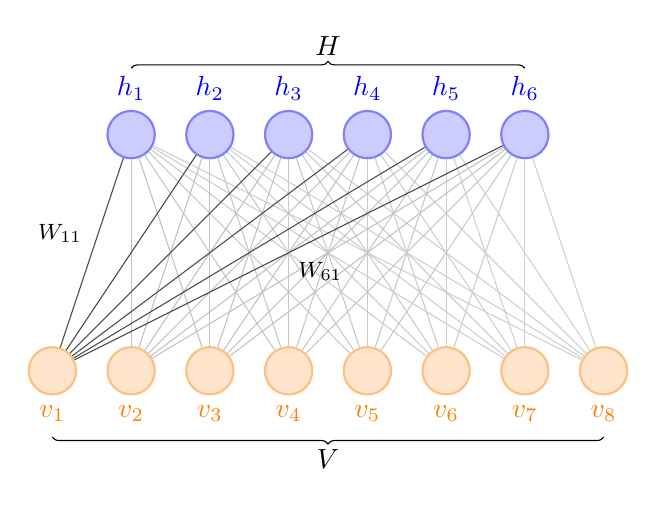
\begin{tikzpicture}
   [
     % $inner sep=2mm,
     hidden/.style={circle,draw=blue!50,fill=blue!20,thick, minimum size=6mm},
    visible/.style={circle,draw=orange!50,fill=orange!20,thick, minimum size=6mm}]
     % draw hidden
     \foreach \x in {1, ...,  6} {
       \node (h\x) at (\x - 3, 3) [hidden,
                               label={[blue]above:$h_{\x}$}] {};
     };
     % draw visible nodes
     \foreach \x in {1, ...,  8} {
       \node (v\x) at (\x-4, 0) [visible,
                               label={[orange]below:$v_{\x}$}] {};
     };
     % draw edges
     \foreach \h in {1, ...,  6} {
       \foreach \v [evaluate=\v as \alpha using 26 - \v  ] in {2, ..., 8} {
            \draw [-, draw=black!\alpha] (v\v) to (h\h);
       }
     };

     \foreach \h in {2, ...,  5} {
       \draw [-, draw=black!70] (v1) to (h\h);
     };
    \draw [-, draw=black!70] (v1) to node [midway, auto, font=\footnotesize] {$W_{11}$} (h1) ;
    \draw [-, draw=black!70] (v1) to node [midway, auto, swap, font=\footnotesize] {$W_{61}$} (h6) ;
    \draw [decorate, decoration={brace, mirror, raise=15pt}] (v1.south) --  node [below=16pt] {$V$} (v8.south);
    \draw [decorate, decoration={brace, raise=15pt}] (h1.north) --  node [above=16pt] {$H$} (h6.north);
 \end{tikzpicture}
\caption{\label{fig:rbm_diagram}A diagram of an RBM with 6 hidden units and 8 visible units.}
\end{figure}


\subsection{RBM as a probability distribution}
\label{sec:org68e304a}

We can consider the RBM as a function on binary strings of length \(N_V\)
\(\rbm: \{0, 1\}^{N_V} \to \mathbb{R}\)

\[
\rbm(\xv) = \sum_{\hv} e^{-E(\xv, \hv)}
\]
RBMs are an energy based model that uses an energy function in determining its output.

Here, \(\vv, \hv\) are binary vectors.


\begin{equation}
E(\vv, \hv) = -\sum_{v = 1}^{N_V} V_v \vv_{v} - \sum_{h = 1}^{N_H} H_h \hv_h - \sum_{v = 1}^{N_V} \sum_{h = 1}^{N_H} \hv_h W_{hv} \vv_v \label{ml:energy}
\end{equation}

Alternatively, Eq. \eqref{ml:energy} can be written as follows when vectorised.

\begin{equation}
E(\vv, \hv) = -V^{T}\vv - H^{T}\hv - \hv^T W \vv
\end{equation}


Probability distribution:
\(
\Pr(\xv) = \frac{1}{Z} \rbm(\xv)
\)

\(
Z = \sum_{\xv} \rbm(X = \xv)
\)
(In the machine learning literature, it is common to use \(\mathbf{a}\) and \(\mathbf{b}\) for the hidden and visible unit weights.)





In order for \(\rbm(\xv)\) to be a probability distribution, it needs to be normalised using the partition function \(Z\).


Indeed, RBM 'learning' consists of adjusting the weights \(W, V, H\) to model a probability distribution.

\subsection{Part 2: RBM learning}
\label{sec:org767671e}

Suppose \(p_{data}(\xv)\) is the target distribution we would like our RBM to learn. Then, training requires a list of \(m\) samples \(\mathbb{X} =  [\xv^{(1)}, \xv^{(2)}, \dots, \xv^{(m)}]\) from \(p_{data}(\xv)\).


Training an


\subsubsection{Simple worked example}
\label{sec:orgcf63d83}

We will go through a simple example of a RBM learning a probability distribution.
Consider the distribution of the sum of two dice rolls. Indeed, this is a binomial distribution.

Fig. \ref{fig:p1-dice} is a plot of the samples, drawn from 10000 trials.




\begin{figure}[htbp]
\centering
\includegraphics[width=.9\linewidth]{/home/frank/shared/quantum/honours-thesis/rbm_learning/p1_dice.png}
\caption{\label{fig:p1-dice}The sum of two dice rolls}
\end{figure}


\section{Burning questions}
\label{sec:orge2c6c1a}
\begin{itemize}
\item Why use the Sigmoid function?
\begin{figure}[htbp]
\centering
\includegraphics[scale=0.2]{/home/frank/shared/quantum/honours-thesis/rbm_learning/rbm_learning.org_20220305_105235_N9II2d.png}
\caption{The Logistic Sigmoid function}
\end{figure}
\end{itemize}

Answer: It's differentiable at non 0 places. Gets infinitely better as it gets closer to 0.

\begin{itemize}
\item Multivariate calculus\ldots{}
\begin{center}
\includegraphics[scale=0.3]{/home/frank/shared/quantum/honours-thesis/rbm_learning/rbm_learning.org_20220305_105553_Ghq5ul.png}
\end{center}
\end{itemize}

\section{Very rough notes}
\label{sec:org5e55b46}
The family of gradient based leaning algorithms commonly used by RBMs is called \emph{Contrastive Divergence}.

\subsection{The RBM itself}
\label{sec:orgfcdf7b8}
Assume your training set of binary images. Then, you can feed your image \(\mathbb{v}\) into the RBM.

\begin{center}
\includegraphics[width=.9\linewidth]{/home/frank/shared/quantum/honours-thesis/rbm_learning/rbm_learning.org_20220302_123159_1KYkb9.png}
\end{center}

Your \(\mathbf{h}\) vectors are binary vectors, and the sum is taken over all possible values of


\subsection{Contrastive Divergence}
\label{sec:org68fbf5e}
Certain models result in an \emph{unnormalised probability distributions} (page 582, textbook), where the total probability is not 1.

\subsubsection{Partition Function}
\label{sec:orgacb1ebe}
To normalise such a distribution \(\tilde{p}(\mathbf{x})\),

\begin{equation}
p(\mathbf{x}) = \frac{1}{Z} \tilde{p}(\mathbf{x})
\end{equation}

And, \(Z\) which is called the \emph{partition function} is defined as follows for continuous variables.

\begin{equation}
Z = \int \tilde{p}(\mathbf{x}) d\mathbf{x}
\end{equation}

Or, for discrete variables

\begin{equation}
Z = \sum_{\mathbf{x}} \tilde{p}(\mathbf{x})
\end{equation}

Note that the argument to \(Z\) is often omitted in the literature.

Usually, it is intractable to compute \(Z\) directly, so an approximation is used.

\begin{Notes}
!Gibbs distribution! -- distribution of product of clique potentials.
\end{Notes}

\section{Machine learning notes}
\label{sec:orgf96dc4d}
Here, I will briefly give the background for machine learning in the context of RBMs.

Machine learning algorithms are used when it is difficult to directly write an algorithm to do some task. For example, computer vision, or speech recognition.


Mathematically, we want some function \(f\) given some input to produce an output, but \(f\) cannot be readily defined so we opt for a (not necessarily probablistic) but 'good enough' model. In this case, it is sensible to choose a family of functions (?) \(f ( x ; \theta )\) parameterised by \(\theta\) as our model. In a sense, a good model will have a good choice of \(f\), in that \(f\) is able to approximate the distribution of our outputs, and a good choice of \(\theta\).

We will start with supervised learning, where we have a set \(X = \{x_1, x_2, \dots, x_k \}\) of \(k\) inputs and \(Y = \{y_1, y_2, \dots, y_k\} \) outputs. Our goal is to find \(f : X \to \hat{Y}\), where \(\hat{Y} = \{ \hat{y}_1, \hat{y}_2, \dots, \hat{y}_k\}\) and for all \(i\), \( f(x_i) = \hat{y}_i \). The hats on the \(Y\)s is to show that this just an approximation for actual \(y\) values. Of course, a good model will be one such that for all \(i\), \(\hat{y}_i \approx y_i\).


\emph{Linear regression} is a good example of a machine learning algorithm.

\subsection{Finding a good parameterisation}
\label{sec:org62e1e7f}
What is a good choice of \(\theta\)? It only makes sense to ask this question if we can measure the performance of a particular choice of \(\theta\). To this end, let \(C(f, \theta)\) be the cost function that produces a scalar output. So now, the best choice of \(\theta\) is one that optimises \(C\).

A simple and commonly used cost function is the mean squared error, \(C(Y, \hat{Y}) = \sum_i (y_i - \hat{y}_i)^2\).



\subsection{Mathematical fundamentals}
\label{sec:orgc973878}
\emph{From scratch} spends a lot of time talking about calculating gradients to functions.

Suppose, \(f : A \to A\), \(g : (A, A) \to A\). Then, given the map \(Z(x, y) = (f \circ g) (x, y)\), we want to find out how the gradient of the output with respect to the input. More precisely, \(\frac{dZ}{dx}\) and \(\frac{dZ}{dy}\).
(This is done using the chain rule).

The backward pass is precisely the act of finding gradients with respect to the input variables.




\section{Understanding: Learning for undirected models}
\label{sec:orge8a0432}
\subsection{Partition Functions}
\label{sec:orge3c30ad}
\subsection{Maximum likelihood}
\label{sec:org3bc2985}
``Negative phase is very hard''. So naive algorithm isn't used.

\subsection{Contrastive Divergence}
\label{sec:org02400d8}
\subsection{Gibbs Sampling}
\label{sec:org7870ee8}



\section{Thinking}
\label{sec:org97e97c5}
\subsection{Why is it hard to draw from RBMs?}
\label{sec:orgfc49b53}
\subsection{What are the common RBM learning algorithms?}
\label{sec:org6e60d2c}
\begin{itemize}
\item Contrastive Divergence
\item Stochastic maximum likelihood
\item Pseudo-likelihood
\end{itemize}
\end{document}
